\documentclass[letter,11pt]{article}
%\documentclass[letter,twoside,11pt]{article}

\usepackage[spanish,es-nodecimaldot]{babel}
\usepackage[utf8]{inputenc}

\usepackage{lmodern}
\usepackage[T1]{fontenc}
\usepackage{textcomp}

\usepackage{graphicx}
\usepackage{pstricks}

\usepackage{anysize}
\marginsize{3cm}{2cm}{2cm}{3cm}

\usepackage{amsmath}
\usepackage{array}
\usepackage{gensymb}
\usepackage{alltt}

\usepackage{fancyhdr}
\usepackage{lastpage}
\pagestyle{fancy}
\fancyhf{}
\fancyhead[LE,RO]{Laboratorio de Física Básica I}
\fancyfoot[CO,CE]{\thepage\ de \pageref{LastPage}}

\special{papersize=215.9mm,279.4mm}

\usepackage[
    pdfauthor={Carlos Eduardo Caballero Burgoa},%
    pdftitle={Laboratorio de Física Básica I},%
    pdfsubject={Movimiento Uniforme},%
    colorlinks,%
    citecolor=black,%
    filecolor=black,%
    linkcolor=black,%
    urlcolor=black,
    breaklinks]{hyperref}
\usepackage{breakurl}

\newcommand{\blankpage}{
\newpage
\thispagestyle{empty}
\mbox{}
\newpage
}

\renewcommand{\arraystretch}{1.2}

\begin{document}

\begin{titlepage}
\begin{center}
{\Large UNIVERSIDAD MAYOR DE SAN SIMÓN}\\
\vspace*{0.15cm}
{\large FACULTAD DE CIENCIAS Y TECNOLOGÍA}\\
\vspace*{0.10cm}
DEPARTAMENTO DE FÍSICA\\
\vspace*{3.0cm}
{\Large \textbf{LABORATORIO DE FÍSICA BÁSICA I}}\\
\vspace*{0.3cm}
{\Large \textbf{PRACTICA No. 5}}\\
\vspace*{3.5cm}
{\Large \textbf{MOVIMIENTO UNIFORME}}\\
\end{center}

\vspace*{7.4cm}
\leftskip=7.95cm
\noindent
\textbf{Estudiante:}\\
Caballero Burgoa, Carlos Eduardo.\\
\newline
\textbf{Docente:}\\
Msc. Guzmán Saavedra, Rocio.\\
\newline
\textbf{Grupo:} N5.\\
\textbf{Fecha de realización:} 17 de Diciembre del 2020.\\
\textbf{Fecha de entrega:} 18 de Diciembre del 2020.\\

\end{titlepage}

\blankpage

\section{Objetivo}
Determinar para un movimiento rectilíneo uniforme (MRU) la relación funcional:
posición en función del tiempo.

\section{Marco teórico}
La relación entre la posición y el tiempo de un móvil que se mueve sobre una
superficie horizontal, libre de rozamiento, con condición inicial $X_0=0$, para
$t_0=0$.

\begin{equation*}
    x = v t
\end{equation*}

La velocidad del móvil es:

\begin{equation*}
    v = \frac{dx}{dt}=constante
\end{equation*}
\begin{equation*}
    v = \frac{\Delta x}{\Delta t}=\frac{X_f-X_0}{t_f-t_0}
\end{equation*}

Para un $t_0=0$ obtenemos:

\begin{equation*}
    x = x_0 + vt
\end{equation*}

\section{Materiales}
\begin{itemize}
\item Simulador «PHET cinemática».
\end{itemize}

\section{Procedimiento}
A continuación se describe el procedimiento experimental que se llevará a
cabo.

\begin{enumerate}
\item Haciendo uso del simulador, tomar datos de posición en función del tiempo,
    una vez establecidos un origen de partida y velocidad aleatoria.
\item Graficar los datos tomados tal que pueda verse la relación funcional entre
    estas variables.
\item Hallar la ecuación de la recta por el método gráfico.
\item Aplicar el método de mínimos cuadrados, para hallar los coeficientes de la
    recta y sus errores.
\item Realizar la interpretación física de los parámetros $A$ y $B$ de la recta.
\end{enumerate}

\section{Tablas de datos y resultados}

\subsubsection{Datos obtenidos}

\begin{center}
\begin{tabular}{|c|>{\centering}m{2.25cm}<{\centering}
                  |>{\centering}m{2.25cm}<{\centering}|}
\hline
\multicolumn{3}{|c|}{\textbf{Tabla \#1: Posición-Tiempo}} \\
\multicolumn{3}{|c|}{\textbf{$X_0 = 0$}} \\
\hline
$i$ & $t_i [s]$ & $x_i [m]$ \tabularnewline \hline
  1 & 0.0 &  0.000 \tabularnewline \hline
  2 & 0.0 &  0.292 \tabularnewline \hline
  3 & 0.1 &  0.583 \tabularnewline \hline
  4 & 0.1 &  0.875 \tabularnewline \hline
  5 & 0.2 &  1.167 \tabularnewline \hline
  6 & 0.2 &  1.458 \tabularnewline \hline
  7 & 0.2 &  1.750 \tabularnewline \hline
  8 & 0.3 &  2.042 \tabularnewline \hline
  9 & 0.4 &  2.625 \tabularnewline \hline
 10 & 0.4 &  2.917 \tabularnewline \hline
 11 & 0.5 &  3.208 \tabularnewline \hline
 12 & 0.5 &  3.500 \tabularnewline \hline
 13 & 0.6 &  4.083 \tabularnewline \hline
 14 & 0.6 &  4.375 \tabularnewline \hline
 15 & 0.7 &  4.667 \tabularnewline \hline
 16 & 0.7 &  4.958 \tabularnewline \hline
 17 & 0.7 &  5.250 \tabularnewline \hline
 18 & 0.8 &  5.542 \tabularnewline \hline
 19 & 0.8 &  5.833 \tabularnewline \hline
 20 & 0.9 &  6.125 \tabularnewline \hline
 21 & 1.0 &  6.708 \tabularnewline \hline
 22 & 1.0 &  7.000 \tabularnewline \hline
 23 & 1,0 &  7.292 \tabularnewline \hline
 24 & 1.1 &  7.583 \tabularnewline \hline
 25 & 1.2 &  8.167 \tabularnewline \hline
 26 & 1.2 &  8.458 \tabularnewline \hline
 27 & 1.2 &  8.750 \tabularnewline \hline
 28 & 1.3 &  9.042 \tabularnewline \hline
 29 & 1.3 &  9.333 \tabularnewline \hline
 30 & 1.4 &  9.625 \tabularnewline \hline
 31 & 1.4 &  9.917 \tabularnewline \hline
 32 & 1.5 & 10.000 \tabularnewline \hline
\end{tabular}
\quad
\begin{tabular}{|c|>{\centering}m{2.25cm}<{\centering}
                  |>{\centering}m{2.25cm}<{\centering}|}
\hline
\multicolumn{3}{|c|}{\textbf{Tabla \#2: Posición-Tiempo}} \\
\multicolumn{3}{|c|}{\textbf{$X_0 = -5 [m]$}} \\
\hline
$i$ & $t_i [s]$ & $x_i [m]$ \tabularnewline \hline
  1 & 0.0 & -5.000 \tabularnewline \hline
  2 & 0.0 & -4.625 \tabularnewline \hline
  3 & 0.1 & -4.250 \tabularnewline \hline
  4 & 0.1 & -3.875 \tabularnewline \hline
  5 & 0.2 & -3.500 \tabularnewline \hline
  6 & 0.2 & -3.125 \tabularnewline \hline
  7 & 0.3 & -2.750 \tabularnewline \hline
  8 & 0.3 & -2.375 \tabularnewline \hline
  9 & 0.4 & -1.625 \tabularnewline \hline
 10 & 0.4 & -1.250 \tabularnewline \hline
 11 & 0.5 & -0.875 \tabularnewline \hline
 12 & 0.5 & -0.500 \tabularnewline \hline
 13 & 0.6 &  0.250 \tabularnewline \hline
 14 & 0.6 &  0.625 \tabularnewline \hline
 15 & 0.7 &  1.000 \tabularnewline \hline
 16 & 0.7 &  1.375 \tabularnewline \hline
 17 & 0.8 &  1.750 \tabularnewline \hline
 18 & 0.8 &  2.125 \tabularnewline \hline
 19 & 0.8 &  2.500 \tabularnewline \hline
 20 & 0.9 &  2.875 \tabularnewline \hline
 21 & 1.0 &  3.625 \tabularnewline \hline
 22 & 1.0 &  4.000 \tabularnewline \hline
 23 & 1.0 &  4.375 \tabularnewline \hline
 24 & 1.1 &  4.750 \tabularnewline \hline
 25 & 1.2 &  5.500 \tabularnewline \hline
 26 & 1.2 &  5.875 \tabularnewline \hline
 27 & 1.3 &  6.250 \tabularnewline \hline
 28 & 1.3 &  6.625 \tabularnewline \hline
 29 & 1.3 &  7.000 \tabularnewline \hline
 30 & 1.4 &  7.375 \tabularnewline \hline
 31 & 1.4 &  7.750 \tabularnewline \hline
 32 & 1.5 &  8.125 \tabularnewline \hline
\end{tabular}
\end{center}

\section{Gráficas}

\subsection{$X_0 = 0$}
Para la tabla \#1 se tiene:

\begin{figure}[!h]
\centering
\includegraphics[scale=1.00]{resources/5.1.eps}
\caption{Gráfica de posición en función del tiempo}
\label{practica51}
\end{figure}

Por la forma de la gráfica \#1 el modelo que se asume para la relación funcional
$x = x(t)$ es:

\begin{equation*}
    x = A + B t
\end{equation*}

\subsubsection{Método gráfico}

Calculando los parámetros $A$ y $B$:

\begin{equation*}
    A = 0
\end{equation*}

\begin{equation*}
    B = \frac{10.0-0}{1.5-0} = \frac{10}{1.5} = 6.6667
\end{equation*}

Por lo que la relación funcional $x = x(t)$ es:

\begin{equation}
    x = 6.67 t
\end{equation}

\subsubsection{Método analítico}

Calculando los valores de la recta por el método de los mínimos cuadrados, se
obtiene:

\begin{equation*}
    A = (0.06 \pm 0.07)[m];117.43\%
\end{equation*}

\begin{equation*}
    B = (6.92 \pm 0.09)[m/s];1.24\%
\end{equation*}

Con los parámetros obtenidos la relación $x = x(t)$ es:

\begin{equation}
    x = 0.06 + 6.92 t
\end{equation}

El significado físico de estos parámetros son que $A = 0.06$ es la posición
inicial $d_0$ cuando el tiempo es $0 [s]$, mientras que $B = 6.92$ representa la
velocidad constante con la que el objeto se desplaza.

\subsubsection{Memoria de calculo}

\paragraph{Entrada del programa}
\begin{alltt}
\footnotesize
\input{resources/i5_1.csv}
\normalsize
\end{alltt}

\paragraph{Comandos del programa}
\begin{alltt}
\footnotesize
\input{resources/p5_1_2.m}
\normalsize
\end{alltt}

\paragraph{Salida del programa}
\begin{alltt}
\footnotesize
\input{resources/o5_1_2.txt}
\normalsize
\end{alltt}

\subsection{$X_0 = -5$}
Para la tabla \#2 se tiene:

\begin{figure}[!h]
\centering
\includegraphics[scale=1.00]{resources/5.2.eps}
\caption{Gráfica de posición en función del tiempo}
\label{practica52}
\end{figure}

Por la forma de la gráfica \#2 el modelo que se asume para la relación funcional
$x = x(t)$ es:

\begin{equation*}
    x = A + B t
\end{equation*}

\subsubsection{Método gráfico}

Calculando los parámetros $A$ y $B$:

\begin{equation*}
    A = -5
\end{equation*}

\begin{equation*}
    B = \frac{8.125+5.0}{1.5-0} = \frac{13.125}{1.5} = 8.750
\end{equation*}

Por lo que la relación funcional $x = x(t)$ es:

\begin{equation}
    x = -5 + 8.75 t
\end{equation}

\subsubsection{Método analítico}

Calculando los valores de la recta por el método de los mínimos cuadrados, se
obtiene:

\begin{equation*}
    A = (-5.01 \pm 0.08)[m];1.72\%
\end{equation*}

\begin{equation*}
    B = (8.9 \pm 0.1)[m/s];1.12\%
\end{equation*}

Con los parámetros obtenidos la relación $x = x(t)$ es:

\begin{equation}
    x = -5.01 + 8.9 t
\end{equation}

El significado físico de estos parámetros son que $A = -5.01$ es la posición
inicial $d_0$ cuando el tiempo es $0 [s]$, mientras que $B = 8.9$ representa la
velocidad constante con la que el objeto se desplaza.

\subsubsection{Memoria de calculo}

\paragraph{Entrada del programa}
\begin{alltt}
\footnotesize
\input{resources/i5_2.csv}
\normalsize
\end{alltt}

\paragraph{Comandos del programa}
\begin{alltt}
\footnotesize
\input{resources/p5_2_2.m}
\normalsize
\end{alltt}

\paragraph{Salida del programa}
\begin{alltt}
\footnotesize
\input{resources/o5_2_2.txt}
\normalsize
\end{alltt}

\section{Cuestionario}
\begin{enumerate}
\item \textbf{¿Cual es la relación $x = x(t)$ obtenida por ambos métodos
    (gráfico y analítico)?}

Se obtienen los siguientes resultados:
\begin{center}
\begin{tabular}{|c|c|}
\hline
\multicolumn{2}{|c|}{$x_0 = 0$} \\
\hline
Método gráfico & $x = 6.67 t$ \\
\hline
Método analítico & $x = 0.06 + 6.92 t$ \\
\hline
\hline
\multicolumn{2}{|c|}{$x_0 = -5$} \\
\hline
Método gráfico & $x = -5 + 8.75 t$ \\
\hline
Método analítico & $x = -5.01 + 8.9 t$ \\
\hline
\end{tabular}
\end{center}

\item \textbf{¿Cual es el significado físico de los parámetros de la ecuación (1)?}

El significado físico de estos parámetros son:

\begin{itemize}
\item Para $x_0 = 0$, se tiene que $A = 0.06$ es la posición inicial $d_0$
cuando el tiempo es $0 [s]$, mientras que $B = 6.92$ representa la velocidad
constante con la que el objeto se desplaza.
\item Para $x_0 = -5$, se tiene que $A = -5.01$ es la posición inicial $d_0$
cuando el tiempo es $0 [s]$, mientras que $B = 8.9$ representa la velocidad
constante con la que el objeto se desplaza.
\end{itemize}

\item \textbf{¿Que tipo de comportamiento presentan los desplazamientos para
    intervalos iguales y sucesivos?}

En ambos casos el desplazamiento va incrementándose linealmente.

\item \textbf{¿Como es la velocidad en este tipo de movimiento?}

La velocidad en ambos casos es constante en el tiempo.

\item \textbf{¿Como son los valores de la velocidad obtenidos por los métodos
    gráfico y analítico?}

Los valores de velocidad son valores positivos que se aproximan a la velocidad
teórica establecida en el simulador.

\item \textbf{¿Se verifica la relación teórica entre la posición y el tiempo del
    movimiento uniforme?}

En ambos casos los valores teóricos de la relación funcional están muy próximos,
siendo el método analítico el que mejor aproximación posee.

\end{enumerate}

\end{document}
